\documentclass[a4paper]{jpconf}
\usepackage[cp1252]{inputenc}
\usepackage{iopams}
\begin{document}
\title{Equation of state for titanium at high energy densities}

\author{K~V~Khishchenko}

\address{Joint Institute for High Temperatures of the Russian Acad\-emy of Sciences, Izhorskaya 13 Bldg~2, Moscow 125412, Russia}

\ead{konst@ihed.ras.ru}

\begin{abstract}
A caloric equation-of-state model, which represents the relation of pressure with density and internal energy, is applied for titanium in the bcc and liquid phases. Thermodynamic characteristics along the cold-compression curve at $T=0$ and Hugoniots are calculated for the metal and compared with available data from shock-wave experiments at high energy densities.
\end{abstract}

\section{Introduction}
Development of new sources of intense pulsed influences on matter (explosives, light-gas guns, lasers, particle accelerators, high electrical current generators) makes demands of hydrodynamic simulations of processes at high energy densities~\cite{Bushman-Fortov-Kanel-Ni-1993, Agureikin-Anisimov-Bushman-Kanel-Karyagin-Konstantinov-Kryukov-Minin-Razorenov-Sagdeev-Sugak-Fortov-HT-1984, Fortov-Kim-Lomonosov-Matveichev-Ostrik-IJImpEng-2006, Povarnitsyn-Khishchenko-Levashov-IJImpEng-2006, Tkachenko-Levashov-Khishchenko-JPA-2006, Oreshkin-Khishchenko-Levashov-Rousskikh-Chaikovskii-HT-2012, Inogamov-Zhakhovsky-Petrov-Khokhlov-Ashitkov-Khishchenko-Migdal-Ilnitsky-Emirov-Komarov-Shepelev-Miller-Oleynik-Agranat-Andriyash-Anisimov-Fortov-CPP-2013, Andreev-Povarnitsyn-Veysman-Faenov-Levashov-Khishchenko-Pikuz-Magunov-Rosmej-Blazevic-Pelka-Schaumann-Schollmeier-Roth-LPB-2015, Senchenko-Belikov-Popov-2015, Mayer-2015, Gnyusov-Rotshtein-Mayer-Rostov-Gunin-Khishchenko-Levashov-2016, Krasyuk-Pashinin-Semenov-Khishchenko-Fortov-2016}. Equation of state (EOS) is a necessary element of such simulations~\cite{Bushman-Fortov-Kanel-Ni-1993}. Consistent theoretical description of material response upon changing the pressure and the density over a broad region from normal values to those under extremely high compression or expansion conditions meets insuperable obstacles because of complex inter-particle interactions in disordered media~\cite{Bushman-Fortov-1983}. Possible model simplifications allow obtaining results, which are valid in bounded domains only~\cite{Levashov-Sinko-Smirnov-Minakov-Shemyakin-Khishchenko-JPCM-2010, Shpatakovskaya-2012, Sinko-Smirnov-Ovechkin-Levashov-Khishchenko-HEDP-2013, Dyachkov-Levashov-2014, Minakov-Levashov-Khishchenko-Fortov-JAP-2014, Kadatskiy-Khishchenko-JPCS-2015}. Alternative approach lies in using semiempirical models~\cite{Zeldovich-Raizer-1967, Fortov-Lomonosov-PhysUsp-2014} those are formulated in the framework of theoretical considerations whereas the model parameters are determined based on experimental data.

Titanium and its alloys are widely used as structural materials in ships, air- and spacecrafts, missiles, etc. EOS for the metal is of interest for simulations of various working regimes under extreme conditions at high mechanical and thermal influences.

In this paper, a semiempirical EOS in a caloric form $P = P(V, E)$ is presented for titanium. Here, $P$ is the pressure, $V=\rho^{-1}$ is the specific volume, $\rho$ is the density, $E$ is the specific internal energy. This EOS provides an adequate description of thermodynamic properties of the metal in the bcc and liquid-phase states over a wide range of densities and pressures. In contrast to the previously known EOS models for titanium \cite{Bushman-Lomonosov-Fortov-1992-metals-eng, Greeff-Trinkle-Albers-Ti-2001, Kerley-Ti-2003, Pecker-Eliezer-Fisher-Henis-Ti-2005, Molodets-Golyshev-Ti-2014}, a polynomial form \cite{Khishchenko-TPL-2004-eng} for the curve of cold compression at $T = 0$ is used.

\section{EOS model}
The EOS model is formulated in the general form as
%
\begin{equation}\label{PVE}
P(V,E)=P_\mathrm{c}(V)+\frac{\Gamma(V,E)}{V}\left[E-E_\mathrm{c}(V)\right],
\end{equation}
%
where $E_\mathrm{c}$ and $P_\mathrm{c}=-\rmd E_\mathrm{c}/\rmd V$ are the cold components of energy and pressure at $T=0$, and $\Gamma$ is a coefficient determining the contribution of thermal components of EOS.

The cold interaction energy in the compression region ($\sigma_\mathrm{c} \geqslant 1$, where $\sigma_\mathrm{c} = V_\mathrm{0c}/V$, $V_\mathrm{0c}$ is the specific volume at $P=0$ and $T=0$) is given by the relation \cite{Khishchenko-TPL-2004-eng}
%
\begin{equation}\label{Ecs1}
E_\mathrm{c}(V) = V_\mathrm{0c} a_0 \ln\sigma_\mathrm{c}-V_\mathrm{0c} \sum_{i=1}^{6} \frac{3a_i}{i} \Big(\sigma_\mathrm{c}^{-i/3}-1 \Big) + V_\mathrm{0c} \sum_{i=1}^{2} \frac{3b_i}{i} \Big(\sigma_\mathrm{c}^{i/3}-1 \Big),
\end{equation}
%
providing for the condition
%
\begin{equation}
E_\mathrm{c}(V_\mathrm{0c}) = 0.\label{E0c}
\end{equation}
%
As can be readily seen, derivation of the energy (\ref{Ecs1}) with respect to volume yields an equation for the pressure $P_\mathrm{c}(V)$, which is analogous to the relation proposed previously \cite{Kalitkin-Govorukhina-1965} as an expansion of the Thomas--Fermi model in powers of the atomic cell radius $r_\mathrm{c}\sim\sigma_\mathrm{c}\!^{-1/3}$.

The value of coefficient $b_2$ in equation~(\ref{Ecs1}) is determined from the condition of coincidence with the model of degenerate ideal Fermi-gas of non-relativistic electrons \cite{Landau-Lifshitz-V-1980-eng} at high compression ratios $\sigma_\mathrm{c} \gtrsim 10^3$--$10^4$,
%
\begin{equation}
b_2=Z^{5/3}\frac{1}{5}\left(3\pi^2\right)^{2/3}a_\mathrm{B}^2E_\mathrm{H}\left(Am_\mathrm{u}V_\mathrm{0c}\right)^{-5/3},
\end{equation}
%
where $E_\mathrm{H}$ is the Hartree energy,
$a_\mathrm{B}$ is the Bohr atomic radius,
$m_\mathrm{u}$ is the atomic mass unit (amu),
$A$ is the atomic mass (in amu),
$Z$ is the atomic number of the element.

In order to find the coefficients $b_1$ and $a_i$ in equation~(\ref{Ecs1}), one need solve the problem of minimization of the root-mean-square deviation of pressure at some values of volume in the range $\sigma_\mathrm{c}=50$--$10^3$ from the results of calculation using the Thomas--Fermi model with quantum and exchange corrections \cite{Kalitkin-Kuzmina-1975-eng} taking into account the conditions for the pressure, bulk modulus and its derivative with respect to pressure at $\sigma_\mathrm{c}=1$:
%
\begin{eqnarray}
P_\mathrm{c}(V_\mathrm{0c})=0,\label{P0c}\\
B_\mathrm{c}(V_\mathrm{0c})=-V\rmd P_\mathrm{c}/\rmd V=B_\mathrm{0c},\label{B0c}\\
B'_\mathrm{c}(V_\mathrm{0c})=\rmd B_\mathrm{c}/\rmd P_\mathrm{c}=B'_\mathrm{0c}\label{B1c}.
\end{eqnarray}
%
The problem of conditional minimization is solved with the introduction of Lagrange factors \cite{Bushman-Fortov-Lomonosov-1991-proc}. The values of the parameters $V_\mathrm{0c}$, $B_\mathrm{0c}$ and $B'_\mathrm{0c}$ are fitted by iterations so as to satisfy under normal conditions the value of specific volume $V_0$ and the values of isentropic compression modulus $B_S=-V(\partial P/\partial V)_S=B_{S0}$ and its pressure derivative $B'_S=\left(\partial B_S/\partial P\right)_S=B'_{S0}$ determined from the data of static and shock compressibility measurements.

The energy on the cold curve in the rarefaction region ($\sigma_\mathrm{c}<1$) is given by the polynomial
%
\begin{equation}\label{Ecs2}
E_\mathrm{c}(V) = V_\mathrm{0c} \bigg(\sigma_\mathrm{c}^m \frac{a_\mathrm{m}}{m} + \sigma_\mathrm{c}^n \frac{a_\mathrm{n}}{n}-\sigma_\mathrm{c}^l \frac{a_\mathrm{m} +a_\mathrm{n}}{l}\bigg) + E_\mathrm{sub},
\end{equation}
%
which provides for the value of the sublimation energy $E_\mathrm{c}=E_\mathrm{sub}$ at $V\to \infty$ as well as for the reference condition~(\ref{P0c}).
The requirement to satisfy equations~(\ref{E0c}), (\ref{B0c}) and (\ref{B1c}) leaves only two free parameters ($l$ and $n$) in equation~(\ref{Ecs2}).

The functional dependence of the coefficient $\Gamma$ upon the volume and internal energy is defined analogously to the caloric model~\cite{Bushman-Fortov-Lomonosov-1991-proc} in the following form:
%
\begin{equation}\label{Gamma}
\Gamma(V,E)=\gamma_\mathrm{i}+\frac{\gamma_\mathrm{c}(V)-\gamma_\mathrm{i}}{1+\sigma^{-2/3}\left[E-E_\mathrm{c}(V)\right]/E_\mathrm{a}},
\end{equation}
%
where $\sigma=V_{0}/V$, $\gamma_\mathrm{c}(V)$ corresponds to the case of low thermal energies, and $\gamma_\mathrm{i}$ characterizes the region of highly heated condensed substance. The anharmonicity energy $E_\mathrm{a}$, which sets the thermal energy of a transition from one limiting case to another, is determined from the results of shock-wave experiments at high pressures.

The volume dependence of the cold component of $\Gamma$ is defined as \cite{Bushman-Lomonosov-Fortov-Khishchenko-Zhernokletov-Sutulov-JETP-1996}
%
\begin{equation}\label{gamma_{c}}
\gamma_\mathrm{c}(V)=2/3+\left(\gamma_\mathrm{0c}-2/3\right)\frac{\sigma_\mathrm{n}^2+\ln^2 \sigma_\mathrm{m}}{\sigma_\mathrm{n}^2+\ln^2 (\sigma/\sigma_\mathrm{m})},
\end{equation}
%
where
%
\begin{equation}\label{gamma_0c}
\gamma_\mathrm{0c}=\gamma_\mathrm{i}+\left(\gamma_0-\gamma_\mathrm{i}\right)\bigg[1+\frac{E_0-E_\mathrm{c}(V_0)}{E_\mathrm{a}}\bigg]^2,
\end{equation}
%
$E_0$ and $\gamma_0$ are the values of specific internal energy and Gr\"uneisen coefficient $\gamma=V(\partial P/\partial E)_V$ under normal conditions. The form of $\gamma_\mathrm{c}(V)$ ensures validity of the condition $\gamma(V_0,E_0)=\gamma_0$, and gives the asymptotic value $\gamma_\mathrm{c}=2/3$ in the limiting cases of low and high compression ratios. The parameters $\sigma_\mathrm{n}$ and $\sigma_\mathrm{m}$ are determined from the requirement of optimum fit to experimental data on shock compressibility of porous samples of a substance in question.


\section{EOS for titanium}

Titanium under atmospheric pressure appears in two solid phases~\cite{Tonkov-1979}. Low-temperature $\alpha$-phase with hexagonal closed-packed (hcp) structure is stable up to 1155~K; high-temperature $\beta$-phase with body-centered cubic (bcc) structure remains stable up to the melting point at 1941~K. Under high pressures, more phases of titanium are observed. At the room temperature, the $\alpha$-phase transforms to the $\omega$-phase with hexagonal structure at pressures from 2.9 to 14.9~GPa depending on the compression conditions \cite{Errandonea-Meng-Somayazulu-Hausermann-PB-2005}. Further increase of pressure at the room temperature leads to transformation of $\omega$ to $\gamma$-phase with orthorhombic structure at $116\pm 4$~GPa~\cite{Vohra-Spencer-PRL-2001}, 117~GPa~\cite{Dewaele-Stutzmann-Bouchet-Bottin-Occelli-Mezouar-PRB-2015} or 128~GPa~\cite{Akahama-Kawamura-LeBihan-PRL-2001}, and of $\gamma$ to $\delta$-phase with another orthorhombic structure (distorted-bcc) at 135~GPa~\cite{Dewaele-Stutzmann-Bouchet-Bottin-Occelli-Mezouar-PRB-2015} or 140~GPa~\cite{Akahama-Kawamura-LeBihan-PRL-2001}. Under higher pressures at room temperature, the $\delta$-phase remains stable at least up to 200~GPa~\cite{Dewaele-Stutzmann-Bouchet-Bottin-Occelli-Mezouar-PRB-2015} and even 220~GPa~\cite{Akahama-Kawamura-LeBihan-PRL-2001}. Melting of the $\beta$-phase is studied up to 120~GPa~\cite{Stutzmann-Dewaele-Bouchet-Bottin-Mezouar-PRB-2015}.

Shock compressibility of titanium is investigated with use of traditional explosive systems up to 0.1~TPa~\cite{Walsh-Rice-McQueen-Yarger-PR-1957, McQueen-Marsh-JAP-1960, McQueen-Marsh-Taylor-Fritz-Carter-1970-proc, LASL-1980}. Higher pressures to 0.3~TPa were achieved with special explosive systems~\cite{Krupnikov-Bakanova-Brazhnik-Trunin-DAN-1963} and two-stage gas gun~\cite{Isbell-Shipman-Jones-1968}. By use of special construction of explosive flyer-acceleration system, titanium was loaded in shock waves up to 0.6~TPa~\cite{Altshuler-Bakanova-Dudoladov-Dynin-Trunin-Chekin-1981}. A hemispherical shell explosive device allowed achieving pressure of 1.3~TPa in the metal~\cite{Trunin-Panov-Medvedev-JETP-Lett-1995}. Highest pressure in titanium under controlled conditions was measured about 13.6~TPa in experiments with strong shock waves from underground nuclear explosion~\cite{Trunin-1994-eng, Trunin-Ilkaeva-Podurets-Popov-Pechenkin-Prokhorov-Sevastyanov-Khrustalev-HT-1994}. Compressibility of porous samples was studied as well~\cite{Trunin-Simakov-Medvedev-HT-1999}.

All early experiments~\cite{Walsh-Rice-McQueen-Yarger-PR-1957, McQueen-Marsh-JAP-1960, Krupnikov-Bakanova-Brazhnik-Trunin-DAN-1963, Isbell-Shipman-Jones-1968} did not show existence of transformation of the $\alpha$-phase. First indication of the phase transformation of titanium in shock waves was obtained in detailed series of measurements~\cite{McQueen-Marsh-Taylor-Fritz-Carter-1970-proc, LASL-1980}. More data in the region of the $\alpha$--$\omega$ phase transformation of shock-compressed titanium were obtained in experiments\cite{Altshuler-Bakanova-Dudoladov-Dynin-Trunin-Chekin-1981}. The $\alpha$--$\omega$ transformation of titanium is analyzed elsewhere~\cite{Greeff-Trinkle-Albers-Ti-2001}.

In this work, the data on shock loading of non-porous samples of the metal above 88~GPa are taken into consideration, which are attributed to the $\beta$ (bcc) and liquid phases. At that, the normal density of the metal is taken as a reference value, $\rho_0=4.504$~g/cm$^3$.

The EOS coefficients for titanium obtained within the framework of the model are as follows:
$V_0 = 0.222$,
$V_\mathrm{0c} = 0.221$,
$a_0 = 154.368$,
$a_1 = 129\,198.249$,
$a_2 =-444\,895.983$,
$a_3 = 733\,767.758$,
$a_4 =-659\,402.98$,
$a_5 = 309\,846.579$,
$a_6 =-59\,693.079$,
$b_1 =-12\,373.923$,
$b_2 = 3399.011$,
$a_\mathrm{m} = 86.627$,
$a_\mathrm{n} =-0.827$,
$m = 2.075$,
$n = 12$,
$l = 1$,
$E_\mathrm{sub} = 9.75$,
$\gamma_\mathrm{0c} = 1.75$,
$\sigma_\mathrm{m} = 0.87$,
$\sigma_\mathrm{n} = 0.5$,
$\gamma_\mathrm{i} = 0.45$ and
$E_\mathrm{a} = 20$.
The units of measure correspond to the initial units of $P = 1$~GPa, $V = 1$~cm$^3$/g and $E = 1$~kJ/g.

Calculated principal Hugoniot of titanium is presented in figure~\ref{fig1} in comparison with data from experiments~\cite{Walsh-Rice-McQueen-Yarger-PR-1957, McQueen-Marsh-JAP-1960, Krupnikov-Bakanova-Brazhnik-Trunin-DAN-1963, Isbell-Shipman-Jones-1968, LASL-1980, Altshuler-Bakanova-Dudoladov-Dynin-Trunin-Chekin-1981, Trunin-Panov-Medvedev-JETP-Lett-1995, Trunin-Simakov-Medvedev-HT-1999, Trunin-1994-eng, Trunin-Ilkaeva-Podurets-Popov-Pechenkin-Prokhorov-Sevastyanov-Khrustalev-HT-1994} over a whole investigated range of shock ($U_\mathrm{s}$) and particle ($U_\mathrm{p}$) velocities.
%
A comparison of calculated Hugoniots for samples of different initial porosity $\rho_0/\rho_{00}$ with experimental data~\cite{Walsh-Rice-McQueen-Yarger-PR-1957, McQueen-Marsh-JAP-1960, Krupnikov-Bakanova-Brazhnik-Trunin-DAN-1963, Isbell-Shipman-Jones-1968, LASL-1980, Altshuler-Bakanova-Dudoladov-Dynin-Trunin-Chekin-1981, Trunin-Panov-Medvedev-JETP-Lett-1995, Trunin-Simakov-Medvedev-HT-1999, Trunin-1994-eng, Trunin-Ilkaeva-Podurets-Popov-Pechenkin-Prokhorov-Sevastyanov-Khrustalev-HT-1994} is presented in figures~\ref{fig2}--\ref{fig4}. Here $\rho_{00}$ is the initial density of samples.

\begin{figure}[t]
\centering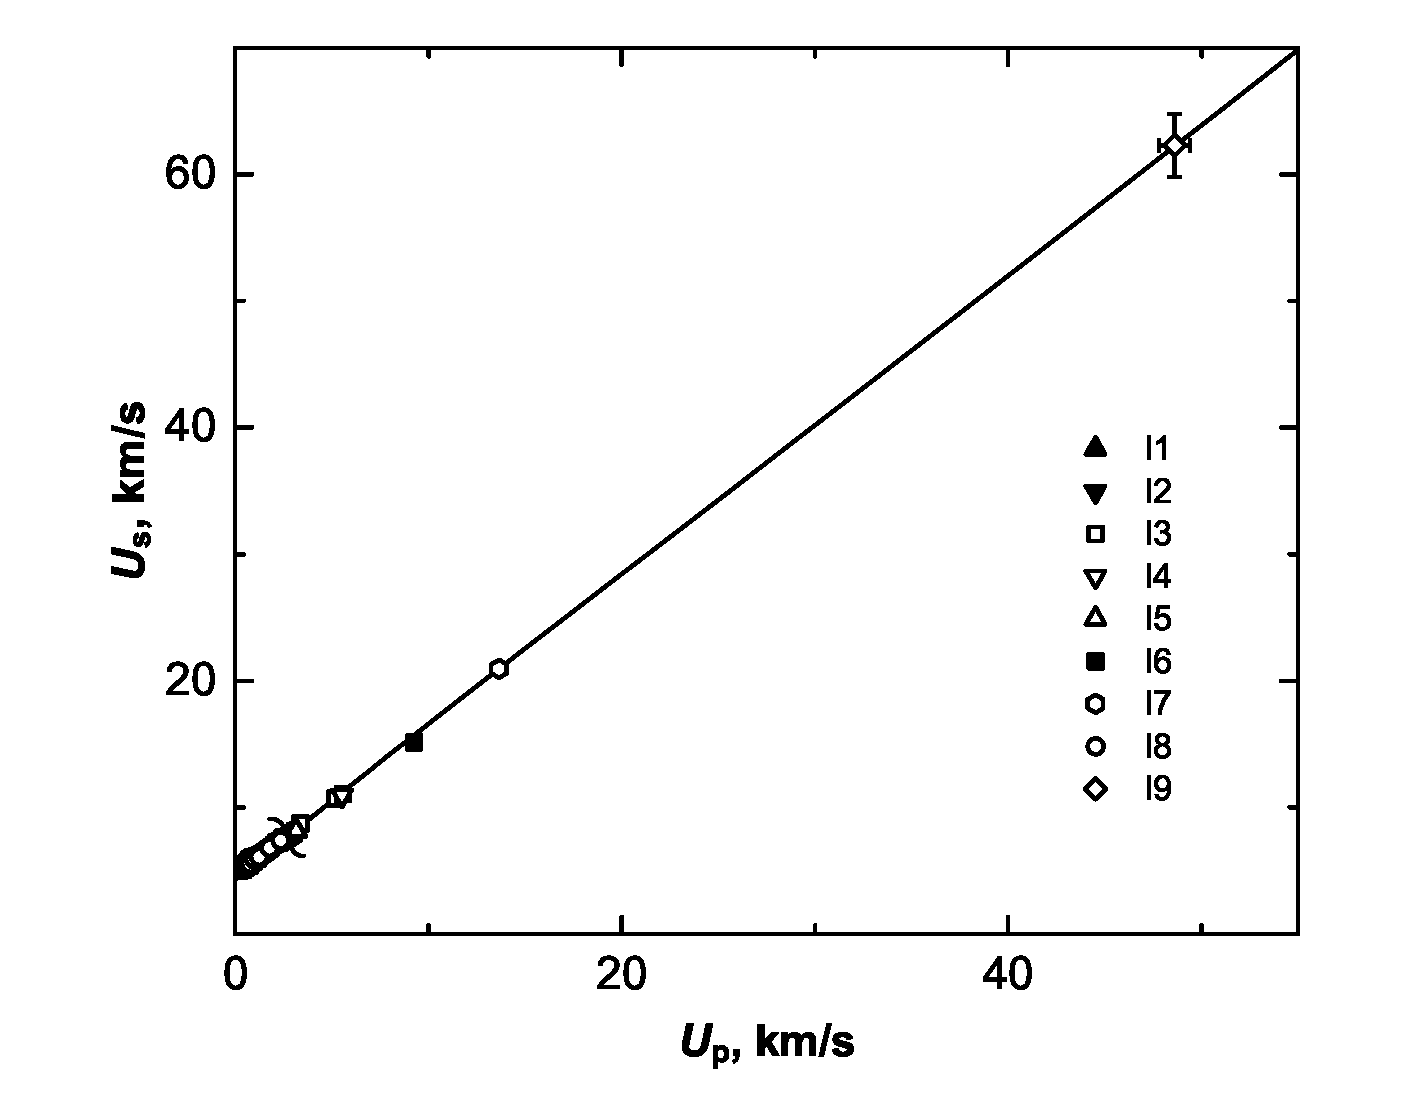
\includegraphics[width=0.76\columnwidth]{fig1.eps}
\caption{The principal Hugoniot of titanium: curve corresponds to the present calculations; wavy line denotes the boundary above which the bcc and liquid phases are described; markers correspond to experimental data
(I1---\!\!\cite{Walsh-Rice-McQueen-Yarger-PR-1957},
I2---\!\!\cite{McQueen-Marsh-JAP-1960},
I3---\!\!\cite{Krupnikov-Bakanova-Brazhnik-Trunin-DAN-1963},
I4---\!\!\cite{Isbell-Shipman-Jones-1968},
I5---\!\!\cite{LASL-1980},
I6---\!\!\cite{Altshuler-Bakanova-Dudoladov-Dynin-Trunin-Chekin-1981},
I7---\!\!\cite{Trunin-Panov-Medvedev-JETP-Lett-1995},
I8---\!\!\cite{Trunin-Simakov-Medvedev-HT-1999},
I9---\!\!\cite{Trunin-1994-eng, Trunin-Ilkaeva-Podurets-Popov-Pechenkin-Prokhorov-Sevastyanov-Khrustalev-HT-1994}).
\label{fig1}
}
\end{figure}

\begin{figure}[t]
\centering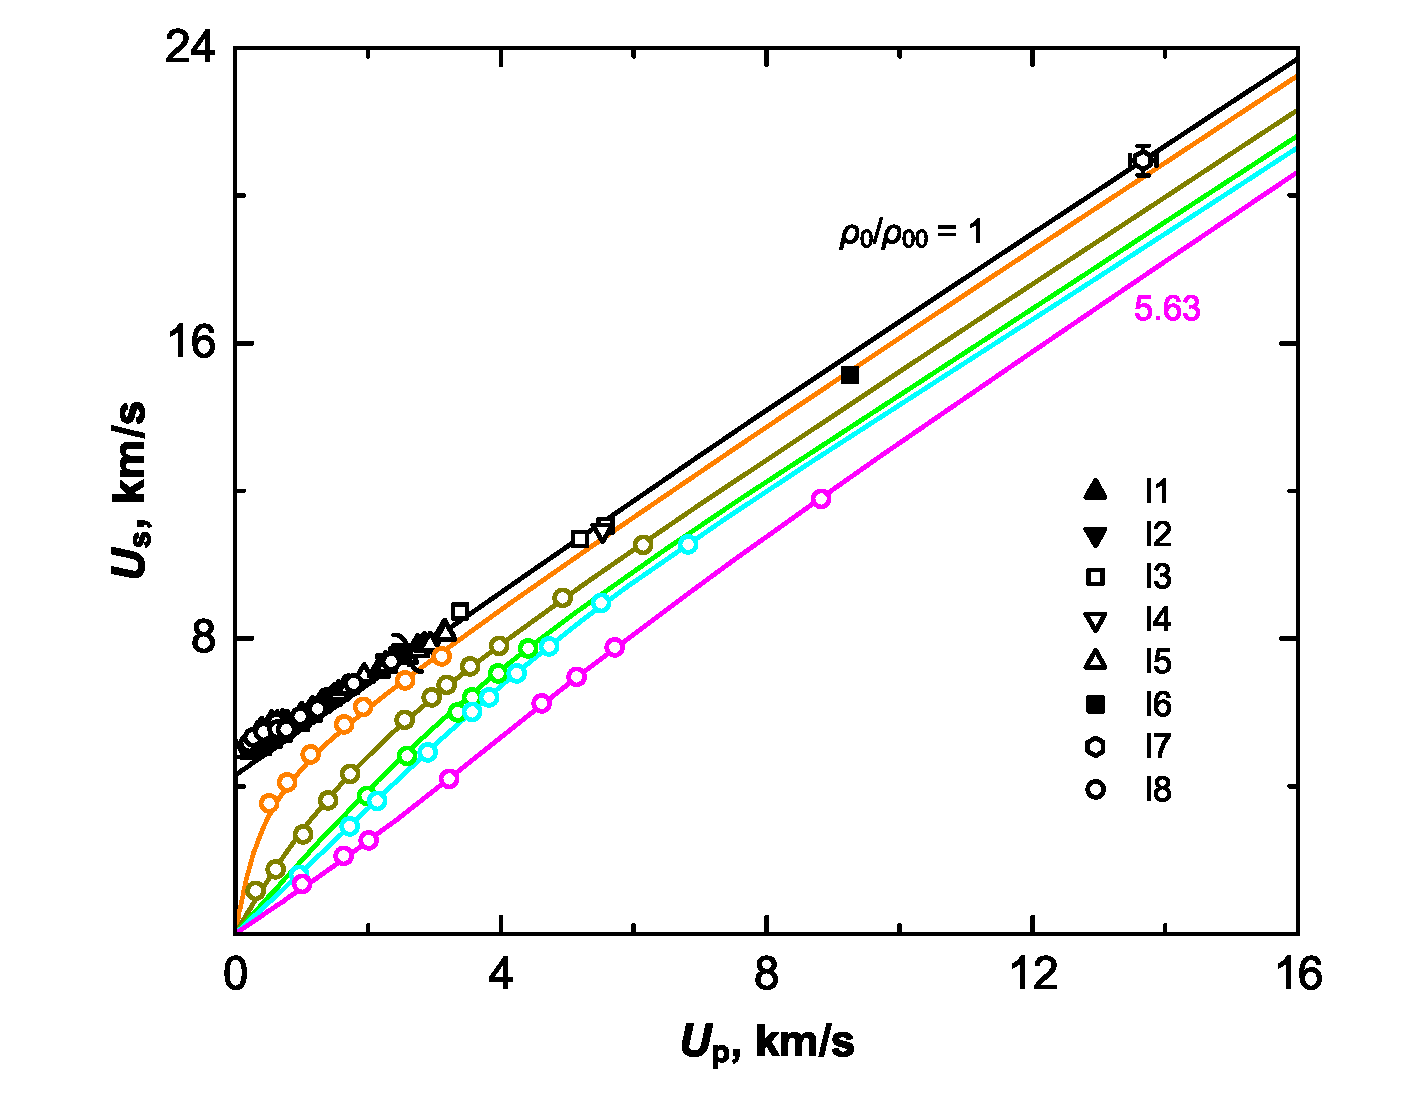
\includegraphics[width=0.76\columnwidth]{fig2.eps}
\caption{The Hugoniots of titanium samples with different initial porosity ($\rho_0/\rho_{00}=1$, 1.12, 1.49, 2, 2.5 and 5.63 for curves top-down respectively): notations are analogous to figure~\ref{fig1}.
\label{fig2}
}
\end{figure}


\begin{figure}[t]
\centering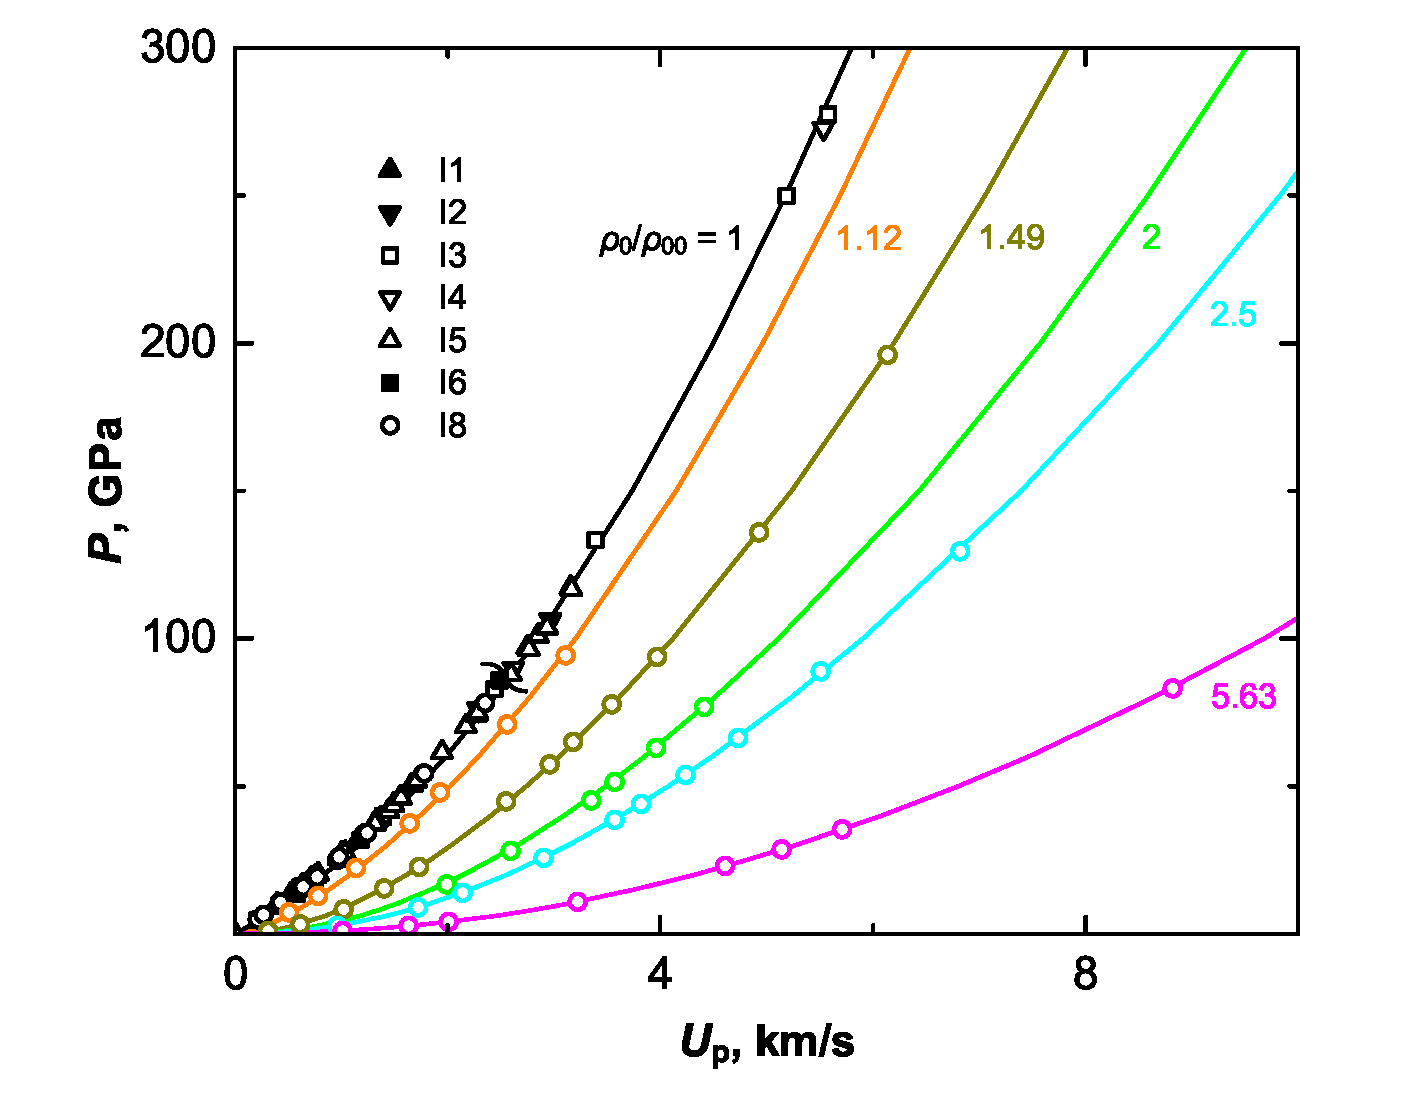
\includegraphics[width=0.76\columnwidth]{fig3.eps}
\caption{The Hugoniots of titanium samples with different initial porosity ($\rho_0/\rho_{00}$): notations are analogous to figure~\ref{fig1}.
\label{fig3}
}
\end{figure}

\begin{figure}[t]
\centering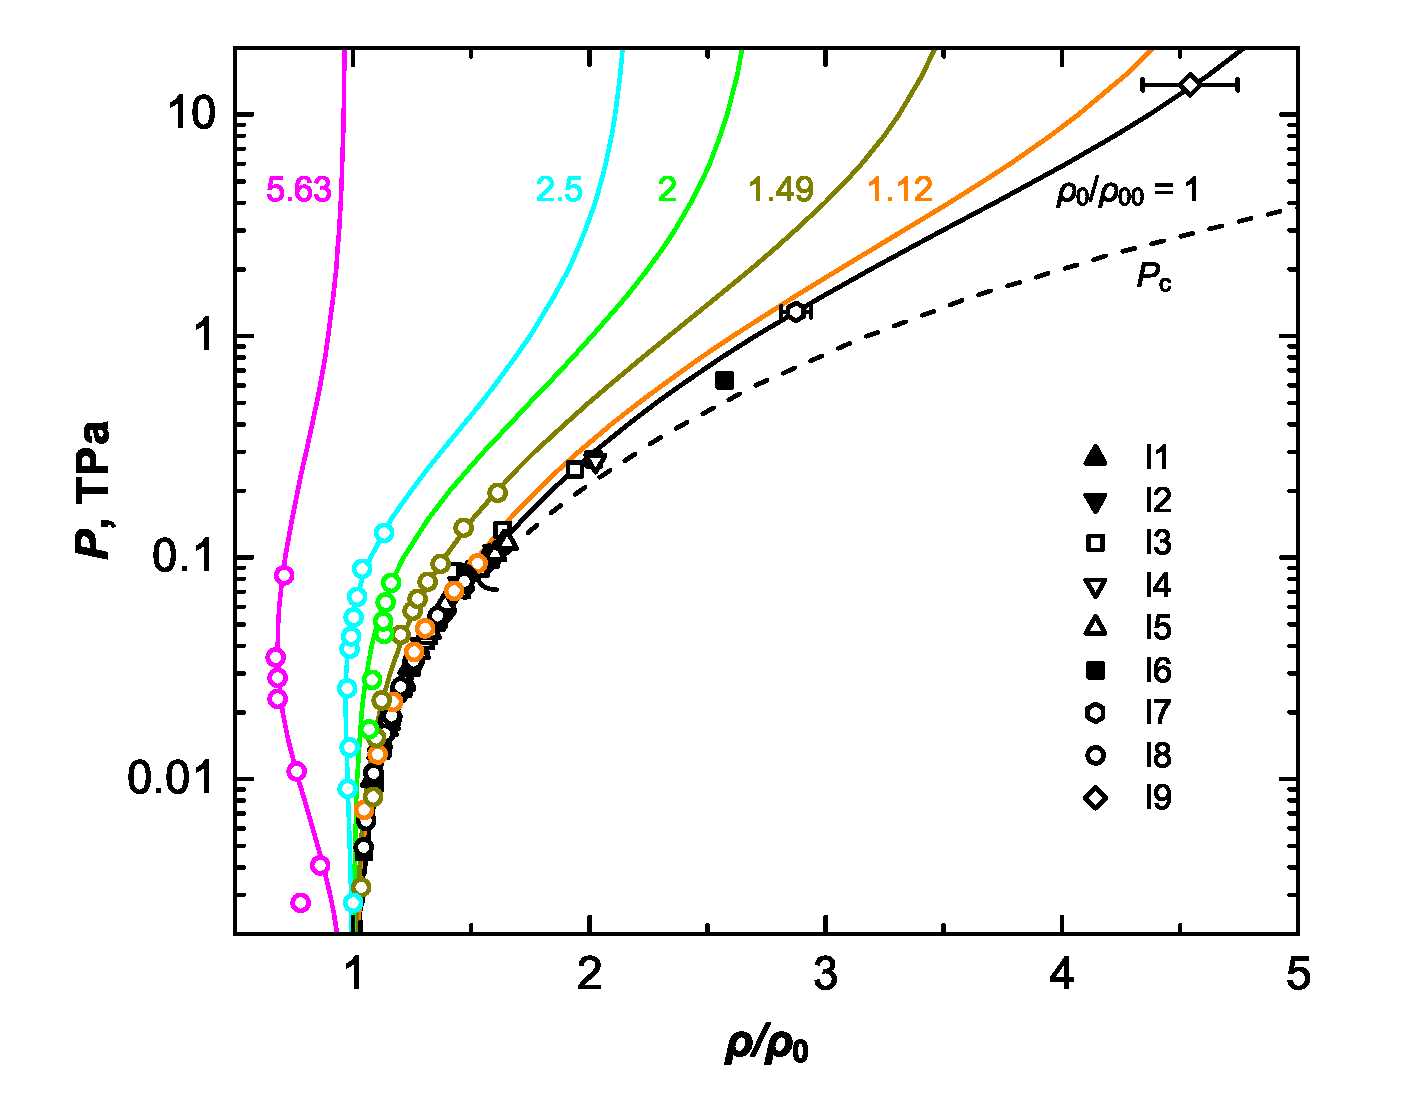
\includegraphics[width=0.76\columnwidth]{fig4.eps}
\caption{The cold curve ($P_\mathrm{c}$) and Hugoniots of tungsten samples with different initial porosity ($\rho_0/\rho_{00}$): notations are analogous to figure~\ref{fig1}.
\label{fig4}
}
\end{figure}

%\clearpage

Calculations of Hugoniots are performed by solving the following equation, which is the law of energy conservation in the shock-wave front~\cite{Zeldovich-Raizer-1967}:
\begin{equation}
E=E_0+\frac{1}{2}(P_0+P)(V_{00}-V),\label{Hug}
\end{equation}
where left-hand side is closed by the EOS, $E=E(P,V)$; $E_0$, $P_0$ and $V_{00}=\rho_{00}\!^{-1}$ are the initial values of specific internal energy, pressure and specific volume of samples; $E_0=E(P_0, V_0)$. Equation \eref{Hug} and the EOS determine the specific volume as a function of pressure along the Hugoniot for samples of initial density $\rho_{00}$.

The laws of conservation of mass and momentum in the shock-wave front~\cite{Zeldovich-Raizer-1967} allow calculating the shock and particle velocities:
\begin{eqnarray}
U_\mathrm{s}=V_{00}\sqrt{(P-P_0)(V_{00}-V)^{-1}},\\
U_\mathrm{p}=\sqrt{(P-P_0)(V_{00}-V)}.
\end{eqnarray}

Analysis of the comparison results in figures~\ref{fig1}--\ref{fig4} shows that the proposed EOS provides for a reliable description of the metal properties in wide ranges of shock and particle velocities, pressures and compression ratios except for the domain of the $\alpha$ and $\omega$ phases (region near the principal Hugoniot below 88~GPa).

Note that the applicability of relation~(\ref{Ecs1}) is restricted to the range of non-relativistic motion of electrons~\cite{Kirzhnits-PhysUsp-1975-eng}: $5Am_\mathrm{u}E_\mathrm{c}/(3Z) \ll m_\mathrm{e}c^2$, where $m_\mathrm{e}$ is the electron mass and $c$ is the speed of light. This condition can be rewritten as $\sigma^{2/3} \ll 2Zm_\mathrm{e}c^2/(5Am_\mathrm{u}V_\mathrm{0c}b_2$), which yields the following limit of applicability with respect to the compression ratio for the cold curve of titanium obtained in this study: $\sigma \ll 10^6$.

It is also needed to note that the pressure $P_\mathrm{c}$ derived from relation~(\ref{Ecs1}) gives result close to that from the adapted polynomial expansion in second order for cold EOS of regular solids~\cite{Holzapfel-EPL-1991, Holzapfel-RPP-1996, Holzapfel-ELBRUS-2010}.

\section{Conclusion}
The unified EOS, which has the form of an analytic function, is proposed for titanium in the bcc and liquid phases. The EOS agrees well with available shock-wave data over a wide range of pressures and compression ratios and may be used effectively in simulations of physical processes in the metal under high-energy-density conditions.

\ack
The author appreciates sincerely Prof Dr Wilfried B Holzapfel for his interest to this approach.
The work is supported by the Russian Science Foundation (grant No.\,14-50-00124).



\section*{References}
\bibliographystyle{iopart-num}
\bibliography{example}

\end{document}